\section{End-User guide}
\subsection{Introduction}
This guide demonstrates how to use our developed application for time series decomposition.
Our demo video can be found at: 
\href{https://www.overleaf.com/learn}{Application Demonstration Video}

\subsection{Quick Start Guide}
This is a quick guide to help a user get started with our application.
\begin{figure}[H]
\centering
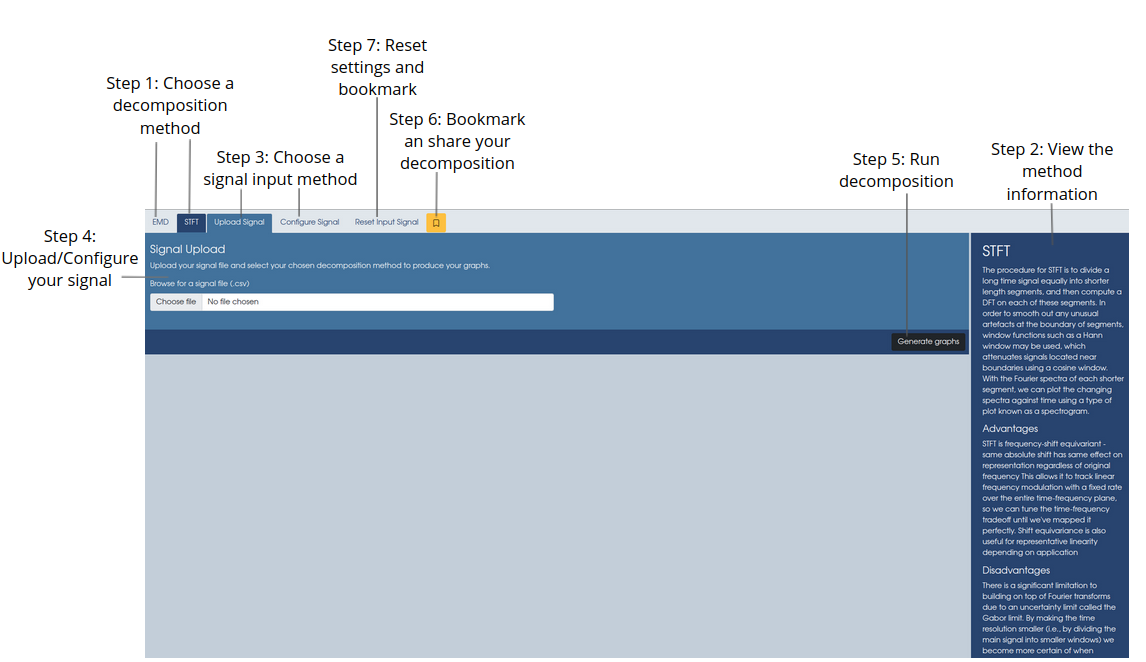
\includegraphics[width=1.0\textwidth]{figures/quickguidesteps.png}
\caption{\label{fig:Application Interface}Application Interface}
\end{figure}


\subsection{User Instructions}
\subsubsection{Configuring a combined signal}
\begin{figure}[H]
\centering
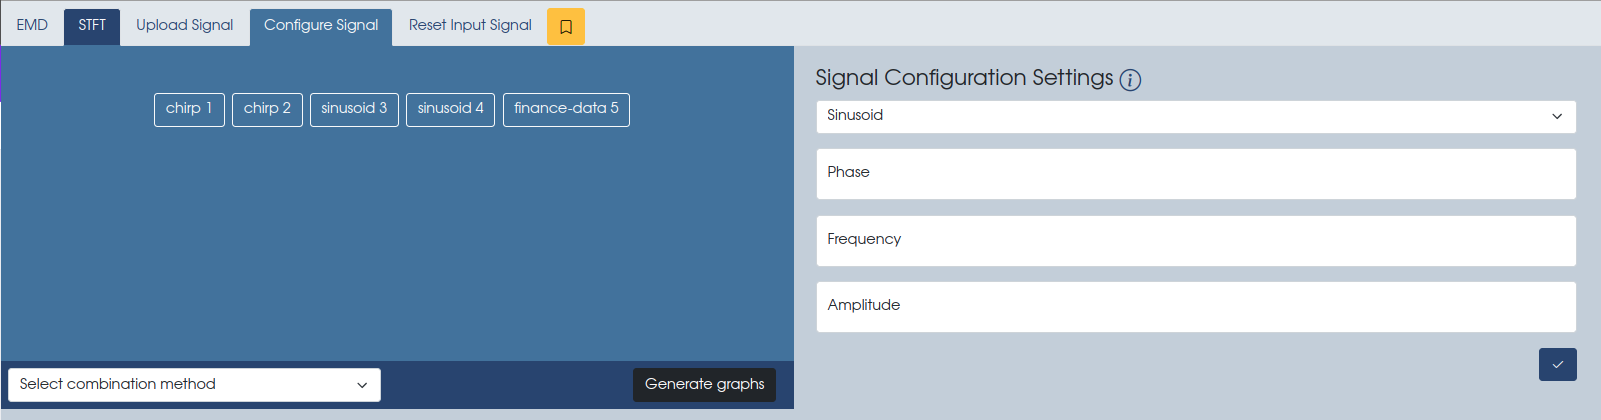
\includegraphics[width=1.0\textwidth]{figures/signalconfig.png}
\caption{\label{fig:Signal Configuration}Signal Configuration}
\end{figure}

\begin{enumerate}
\item Click on the configure signal tab found on the top panel.
\item Select a signal type from the drop down in the 'Signal Configuration Settings' panel.
\item Input your values into the various fields.
\item Press the tick button to add your signal. Your signal should appear on the left hand panel.
\item To edit or delete your signal, click on the signal and make changes or delete in the 'Signal Configuration Settings' panel.
\item Set your combination method for your signals. Note: only sinusoids and trends should be combined using product method.
\end{enumerate}

\subsubsection{Uploading a signal}
\begin{figure}[H]
\centering
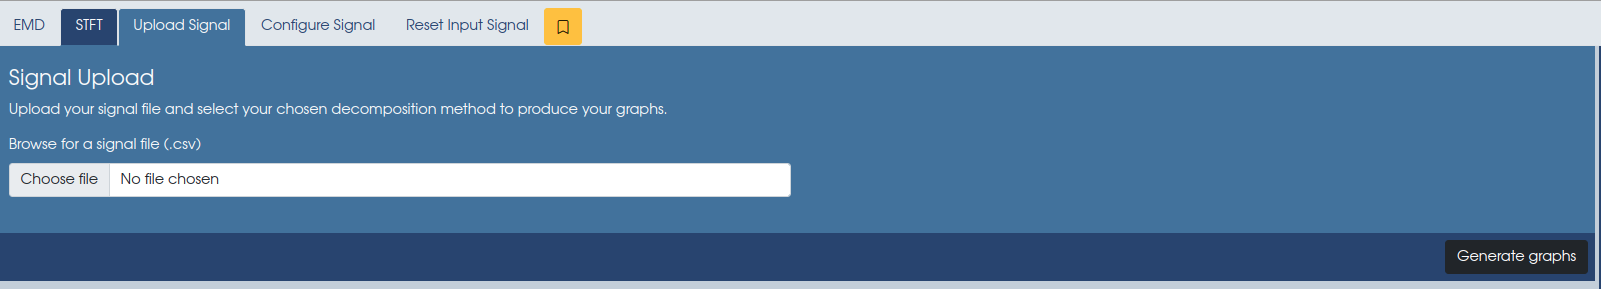
\includegraphics[width=1.0\textwidth]{figures/signalupload.png}
\caption{\label{fig:Signal Upload}Signal Upload}
\end{figure}

\begin{enumerate}
\item Click on the upload signal tab found on the top panel.
\item Choose a file to upload. Note: Only .csv files are currently supported.
\item You should receive an upload complete message if the upload was a success.
\end{enumerate}

\subsubsection{Selecting decomposition method}
\begin{enumerate}
\item Click on either the 'EMD' or 'STFT' tab on the top panel to select a method. An information panel will open up on the right hand side.
\item EMD (Empirical Mode Decomposition): This method will result in various IMF (Intrinsic Mode Function) graphs %and a Hibert-Huang Spectrum  
\item STFT: This method will result in an FFT (Fast Fourier Transform) graph and a resultant spectrogram.
\end{enumerate}

\subsubsection{Running decomposition method}
\begin{enumerate}
\item Once you have completed configuring your settings, click on 'Generate graphs'.
\item Your decomposition graphs should appear below the settings panel. This may take a couple of minutes based on your settings.
\item You may click on your charts on the left hand panel to expand them into the larger view area.
\end{enumerate}

\subsubsection{Bookmarking}
\begin{enumerate}
\item Once you have completed configuring your settings, simply click on the yellow bookmark button.
\item Your settings will be saved into your URL and your URL is now copied to your clipboard and can be pasted anywhere.
\item You should now be able to access your settings in a different window by pasting the URL into the address bar.
\end{enumerate}
